\section{Evaluación del modelo mediante casos hipotéticos}\label{sec:evalmodel-casoshipot}

% Descripción de los tipos de cuarentena y las medidas de cuidado 
Las combinaciones entre los distintos niveles de cuidado y cuarentena presentados en \ref{met:evaluacion} dan lugar a una serie de casos, los cuales son presentados en la tabla \ref{table:casos-hipoteticos}. Se resuelve el sistema de ecuaciones diferenciales ordinarias \ref{eq:modelo-final} para cada caso, utilizando las distintas variantes de \(\alpha_i(t)\) y \(P(t)\), modificadas a partir de las estimaciones logradas en la sección anterior.

\begin{table}[h!]
\centering
\begin{tabular}{||l| c c c||} 
 \hline
 & \textbf{Cuidado insuficiente} & \begin{tabular}{@{}c@{}}\textbf{Cuidado} \\ \textbf{normal}\end{tabular} & \begin{tabular}{@{}c@{}}\textbf{Cuidado} \\ \textbf{extra}\end{tabular}\\ 
 \hline
 \textbf{Sin cuarentena} & Caso 1 & Caso 2 & Caso 3 \\ 
 \textbf{Cuarentena normal} & Caso 4 & Caso 5 & Caso 6 \\
 \textbf{Cuarentena fuerte} & Caso 7 & Caso 8 & Caso 9 \\
 \hline
\end{tabular}
\caption{Casos hipotéticos para distintas combinaciones de cuarentena y cuidado.}
\label{table:casos-hipoteticos}
\end{table}


Se prueban dos escenarios. En el primero de ellos, \(\beta_{\text{exterior}}\) es un valor mucho más grande que \(1\), de forma que la tasa de contagio está totalmente dominada por el ambiente exterior y prácticamente todos los contagios ocurren fuera de casa. Este se estudia en la subsección \ref{eval:beta-grande}. Este escenario, como se mencionó en la sección \ref{subsec:eleccion-clases-ambientes}, no es consistente con la realidad, puesto que aproximadamente un tercio de los casos se contagia en el hogar \cite{Ferguson2020}. En el segundo escenario, \(\beta_{\text{exterior}}\) es un valor mayor pero cercano a \(1\), de tal forma que el ambiente hogar contribuye a la tasa de contagios, lo que es más realista. Este se estudia en \ref{eval:beta-chico}.


\subsection{Escenario con contagio exterior predominante}\label{eval:beta-grande}


En este escenario se considera \(\beta_{\text{exterior}} >> 1\), de forma que la tasa de contagio está totalmente dominada por el ambiente exterior y las infecciones ocurren solamente en el exterior del hogar, las infecciones dentro del hogar son despreciables en comparación. Se utiliza \(\beta_{\text{exterior}} = 68.0\), pero los resultados son similares para un rango amplio de parámetros.

% Las figuras \ref{img:all-hip-S-N} y \ref{img:all-hip-I-N} presentan la evolución de los susceptibles \(S_i/N_i\) e infectados \(S_i/N_i\) (normalizados por el total de personas en cada clase), para cada uno de los casos. Se utilizan los mismos límites para los ejes \(y\) para facilitar la comparación.

Como era de esperarse, las diferencias socioeconómicas en la incidencia disminuyen debido a que la mayoría de los casos están utilizando, o bien la misma matriz de tiempos de residencia, o bien los mismos factores sanitarios, o incluso ambos.

La tabla \ref{table:descripcion-casos-hipot} describe los resultados para los distintos casos considerados, tomando como referencia el caso 5, de cuarentena y cuidado normal. En los casos 1 y 2, que corresponden a casos sin cuarentena con cuidado insuficiente o cuidado normal respectivamente, se contagia la gran mayoría de la población dentro de los primeros 6 meses considerados. En el caso con cuidado normal, la clase más acomodada resulta tener una incidencia bastante menor que las demás.

El cuidado extra logra contener la enfermedad con cuarentena normal o fuerte, como muestran los casos 6 y 9. La enfermedad desaparece rápidamente de entre la población en los primeros meses, aunque esto desde luego no considera importación de casos externos.

\begin{table}[H]
\centering
\begin{tabular}{||m{2.5cm}|m{4cm} m{4cm} m{4cm}||} 
 \hline
 & \begin{tabular}{@{}c@{}}\textbf{Cuidado} \\ \textbf{insuficiente}\end{tabular} & \begin{tabular}{@{}c@{}}\textbf{Cuidado} \\ \textbf{normal}\end{tabular} & \begin{tabular}{@{}c@{}}\textbf{Cuidado} \\ \textbf{extra}\end{tabular}\\ 
 \hline
 \textbf{Sin cuarentena} & \textit{Caso 1}: Se contagia un \(90\%\) de la población en los primeros 6 meses, de manera uniforme entre las distintas clases. Luego la enfermedad desaparece. & \textit{Caso 2}: Se contagia un \(65\%\) de la población de la clase alta en los primeros 6 meses, y un \(80\%\) de las demás clases. Luego la enfermedad desaparece. & \textit{Caso 3}: Se logra controlar el alza de casos, alcanzando el \textit{peak} de mediados de julio de 2020 y el de inicios de mayo de 2021 con menos de la mitad de casos, e incluso se evita el rebrote de junio de 2021. Ver figura \ref{img:esc-beta-grande-c3}.\\ 
 \textbf{Cuarentena normal} & \textit{Caso 4}: El primer \textit{peak} de julio de 2020 alcanza más del doble de casos y tiene una reducción lenta, de tal forma que el \textit{peak} de mayo de 2021 es apenas registrado como un alza ligera. Ver figura \ref{img:esc-beta-grande-c4}. & \textit{Caso 5}: Desarrollo real de la pandemia, tomado como referencia& \textit{Caso 6}: La enfermedad alcanza un pequeño \textit{peak} en julio de 2020 y luego se extingue.\\
 \textbf{Cuarentena fuerte} & \textit{Caso 7}: El primer \textit{peak} es muy similar en fecha y número de infectados, pero con un alza sostenida en el número de casos a partir septiembre de 2020, llegando a un \textit{peak} de más del doble de infectados en julio de 2021.  Ver figura \ref{img:esc-beta-grande-c7}. & \textit{Caso 8}: Se observan dos \textit{peaks} de unas 5000 personas, similar al Caso 3 pero sin poder contener el rebrote de junio de 2021. Ver figura \ref{img:esc-beta-grande-c8}. & \textit{Caso 9}: La enfermedad se extingue luego de los primeros meses. \\
 \hline
\end{tabular}
\caption{Observaciones para cada caso hipotético, escenario con \(\beta_{\text{exterior}} = 68\).}
\label{table:descripcion-casos-hipot}
\end{table}




% Aquí pongo todos los resultados de casos hipotéticos que obtuve... cuarentenas fuertes, etc... 
% \begin{figure}[h]
% \centering
% \includegraphics[width=0.99\textwidth]{img/resultados/allhipcases_S-N_commonylim0_1\parameterstring}
% \caption{Estimación de susceptibles, normalizados por el total de cada grupo \(S_i/N_i\), para cada caso hipotético.}
% \label{img:all-hip-S-N}
% \end{figure}

% \begin{figure}[h]
% \centering
% \includegraphics[width=0.99\textwidth]{img/resultados/allhipcases_I-N_commonylim0-015\parameterstring}
% \caption{Estimación de infectados normalizados por el total de cada grupo \(I_i/N_i\), para cada caso hipotético.}
% \label{img:all-hip-I-N}
% \end{figure}

La figura \ref{img:hip-3478-I-comp} muestra cuatro casos interesantes, comparándolos con la situación normal. En estos tres casos, el impacto es mayor sobre la clase 5 (prioridad alta, la más vulnerable). Esto puede atribuirse al hecho de que esa es la clase que presenta en general un mayor factor sanitario y movilidad, por lo que se verían más favorecidos si pudieran guardar las cuarentenas o las medidas de cuidado de mejor manera.
 
 El caso 3, que puede verse en \ref{img:esc-beta-grande-c3}, es interesante, ya que propone que la pandemia pudo controlarse incluso sin cuarentenas ni reducciones de movilidad, siempre y cuando todos pudieran guardar adecuadamente las distintas medidas de cuidado, evitando aglomeraciones, usando mascarilla, practicando el lavado de manos frecuente, etc. El caso 4, en la figura \ref{img:esc-beta-grande-c4}, coincide en que las medidas de higiene y cuidado fueron importantes, y plantea que evitaron un \textit{peak} de más del doble de casos en los primeros meses de la pandemia. 
 
 
El caso 7, en la figura \ref{img:esc-beta-grande-c7}, afirma que una cuarentena más fuerte habría compensado una falta de preocupación o capacidad de cumplimiento de las medidas de higiene y cuidado, al menos en los primeros meses. La situación se desborda a medida que se acerca el 2021, debido a que la población sale del confinamiento. El caso 8, en la figura \ref{img:esc-beta-grande-c8}, es muy similar al caso 3, pero no logra evitar un segundo \textit{peak} en julio de 2021.

% Fechas 
% important_dates = [
%    Date(2020, 5, 13), # cuarentena total en la RM
%    Date(2020, 10, 25), # plesbicito por nueva constitución
%    Date(2021, 1, 4), # comienza a regir el permiso de vacaciones
%    Date(2021, 2, 1), # comienza un plan de vacunación más fuerte (según datos)
%    Date(2021, 5, 26) # un 50% de la población de Santiago tiene la primera dosis
%]
% casos interesantes: 3, 4, 7, 8

\begin{figure}[H]
     \centering
     \begin{subfigure}[b]{.47\textwidth}
         \centering
         \includegraphics[width=\textwidth]{img/resultados/comparecase_3withnormal_I_\parameterstring}
         \caption{Caso \(3\): Cuidado extra sin cuarentena.}
         \label{img:esc-beta-grande-c3}
     \end{subfigure}
     \hfill
     \begin{subfigure}[b]{.47\textwidth}
         \centering
         \includegraphics[width=\textwidth]{img/resultados/comparecase_4withnormal_I_\parameterstring}
         \caption{Caso \(4\): Cuidado insuficiente y cuarentena normal.}
         \label{img:esc-beta-grande-c4}
     \end{subfigure}
     \hfill
     \begin{subfigure}[b]{.47\textwidth}
         \centering
         \includegraphics[width=\textwidth]{img/resultados/comparecase_7withnormal_I_\parameterstring}
         \caption{Caso \(7\): Cuidado insuficiente y cuarentena fuerte.}
         \label{img:esc-beta-grande-c7}
     \end{subfigure}
     \hfill
     \begin{subfigure}[b]{.47\textwidth}
         \centering
         \includegraphics[width=\textwidth]{img/resultados/comparecase_8withnormal_I_\parameterstring}
         \caption{Caso \(8\): Cuidado normal y cuarentena fuerte.}
         \label{img:esc-beta-grande-c8}
     \end{subfigure}
     \hfill 
    \begin{subfigure}[b]{0.99\textwidth}
    \centering
    \scalebox{0.7}{
    \begin{tikzpicture}
	\begin{pgfonlayer}{nodelayer}
		\node [style=none] (50) at (5, 0) {};
		\node [style=none] (51) at (7, 0) {};
		\node [style=none] (52) at (6, -0.5) {Prioridad Alta};
		\node [style=none] (53) at (2, 0) {};
		\node [style=none] (54) at (4, 0) {};
		\node [style=none] (55) at (3, -0.5) {Prioridad};
		\node [style=none] (56) at (-1, 0) {};
		\node [style=none] (57) at (1, 0) {};
		\node [style=none] (58) at (0, -0.5) {Prioridad};
		\node [style=none] (59) at (-4, 0) {};
		\node [style=none] (60) at (-2, 0) {};
		\node [style=none] (61) at (-3, -0.5) {Prioridad Baja};
		\node [style=none] (62) at (-7, 0) {};
		\node [style=none] (63) at (-5, 0) {};
		\node [style=none] (64) at (-6, -0.5) {Sin Prioridad};
		\node [style=none] (65) at (0, -1) {Media Baja};
		\node [style=none] (66) at (3, -1) {Media Alta};
	\end{pgfonlayer}
	\begin{pgfonlayer}{edgelayer}
		\draw [style=class5] (50.center) to (51.center);
		\draw [style=class1] (62.center) to (63.center);
		\draw [style=class2] (59.center) to (60.center);
		\draw [style=class3] (56.center) to (57.center);
		\draw [style=class4] (53.center) to (54.center);
	\end{pgfonlayer}
\end{tikzpicture}

    }
    \end{subfigure}
        \caption[Personas infectadas para casos hipotéticos seleccionados. Escenario \(\beta_{\text{exterior}} >> 1\).]{Personas infectadas para caso hipotéticos seleccionados, con la estimación de los casos reales de fondo. Diferentes límites para el eje \(y\). Las líneas grises corresponden a las fechas relevantes de la tabla \ref{table:fechas-relevantes}.}
        \label{img:hip-3478-I-comp}
\end{figure}


\subsection{Escenario con contagio en hogar}\label{eval:beta-chico}


En este caso se buscó un valor donde existiera tanto contagio en el hogar como en el exterior; esto se hizo estudiando las contribuciones de los ambientes a la tasa de contagio, calculando las contribuciones a la derivada de cada ambiente dadas por \ref{eq:contribuciones-j}, en la subsección \ref{met-subsec:fijos}, y verificando que las del hogar no fueran despreciables en comparación a las del exterior. El valor elegido fue \(\beta_{\text{exterior}} = 1.2\).

Bajo estas condiciones, se observa que la cuarentena prácticamente no influye en el número de contagios; lo que realmente determina si se controla o no la pandemia es el factor sanitario. Los resultados se sintetizan en la tabla \ref{table:descripcion-casos-hipot-beta-1-2}, y los casos de interés elegidos anteriormente se presentan en la figura \ref{img:hip-3478-I-comp-beta1-2}. Con cuidado extra es posible controlar completamente la pandemia, incluso sin cuarentena. Este modelo, sin embargo, dice que la cuarentena no tuvo ningún impacto, y que bastaban las medidas de cuidado. Finalmente, este modelo predice que si toda la población se hubiera visto enfrentada al mismo riesgo que la clase más vulnerable, la pandemia habría sido muchísimo más grave, alcanzando \textit{peaks} de más del doble de casos.



\begin{table}[h!]
\centering
\begin{tabular}{||m{2.5cm}|m{4cm} m{4cm} m{4cm}||} 
 \hline
 & \begin{tabular}{@{}c@{}}\textbf{Cuidado} \\ \textbf{insuficiente}\end{tabular}  & \begin{tabular}{@{}c@{}}\textbf{Cuidado} \\ \textbf{normal}\end{tabular} & \begin{tabular}{@{}c@{}}\textbf{Cuidado} \\ \textbf{extra}\end{tabular}\\ 
 \hline
 \textbf{Con o sin cuarentena} & \textit{Casos 1, 4 y 7}: Se observan \textit{peaks} de más del doble de casos que el normal, y que se reducen más lentamente. El número de contagios no baja del \(0.5\%\) de la población. Ver figuras \ref{img:esc-beta-chico-c4} y \ref{img:esc-beta-chico-c7}. & \textit{Caso 2 y 8} Muy similares al caso 5, el normal usado como referencia. Ver figura \ref{img:esc-beta-chico-c8}. & \textit{Caso 3, 6, y 9}: La enfermedad tiene un pequeño \textit{peak} en torno a julio de 2020 y se extingue luego de unos meses. Ver figura \ref{img:esc-beta-chico-c3}. \\
 \hline
\end{tabular}
\caption[Observaciones para cada caso hipotético, escenario con \(\beta_{\text{exterior}} = 1.2\)]{Observaciones para cada caso hipotético, escenario con \(\beta_{\text{exterior}} = 1.2\). Tabla condensada, puesto que no hay variaciones importantes con respecto a la fuerza de la cuarentena.}
\label{table:descripcion-casos-hipot-beta-1-2}
\end{table}



\begin{figure}
     \centering
     \begin{subfigure}[b]{.47\textwidth}
         \centering
         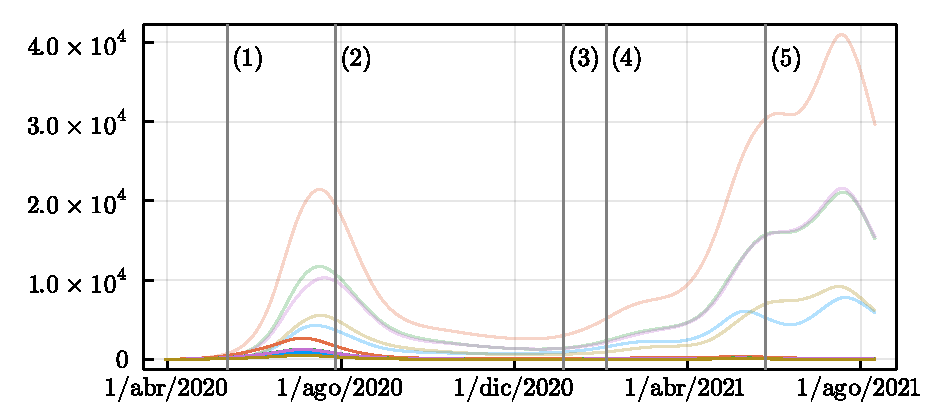
\includegraphics[width=\textwidth]{img/resultados/comparecase_3withnormal_I_gamma_e_0-1724_gamma_i_0-0833_beta_2_2-0000.pdf}
         \caption{Caso \(3\): Cuidado extra sin cuarentena.}
         \label{img:esc-beta-chico-c3}
     \end{subfigure}
     \hfill
     \begin{subfigure}[b]{.47\textwidth}
         \centering
         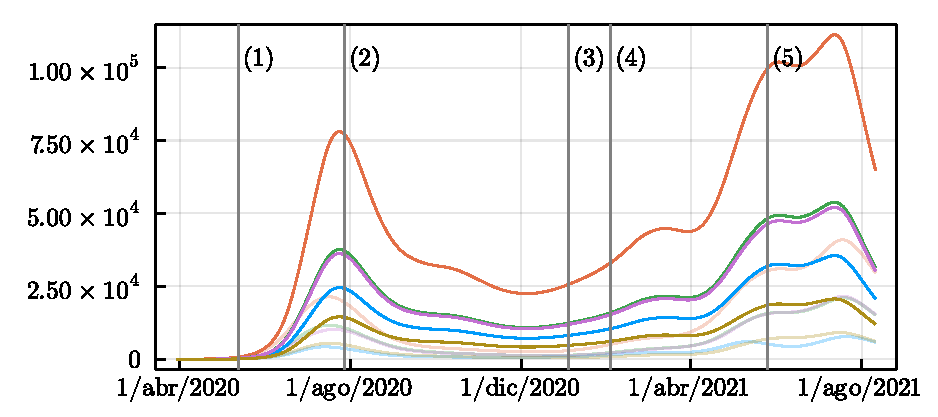
\includegraphics[width=\textwidth]{img/resultados/comparecase_4withnormal_I_gamma_e_0-1724_gamma_i_0-0833_beta_2_2-0000.pdf}
         \caption{Caso \(4\): Cuidado insuficiente y cuarentena normal.}
         \label{img:esc-beta-chico-c4}
     \end{subfigure}
     \hfill
     \begin{subfigure}[b]{.47\textwidth}
         \centering
         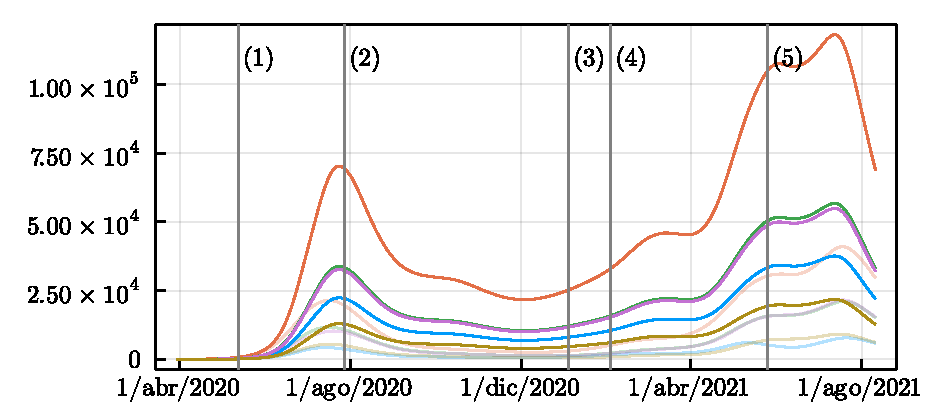
\includegraphics[width=\textwidth]{img/resultados/comparecase_7withnormal_I_gamma_e_0-1724_gamma_i_0-0833_beta_2_2-0000.pdf}
         \caption{Caso \(7\): Cuidado insuficiente y cuarentena fuerte.}
         \label{img:esc-beta-chico-c7}
     \end{subfigure}
     \hfill
     \begin{subfigure}[b]{.47\textwidth}
         \centering
         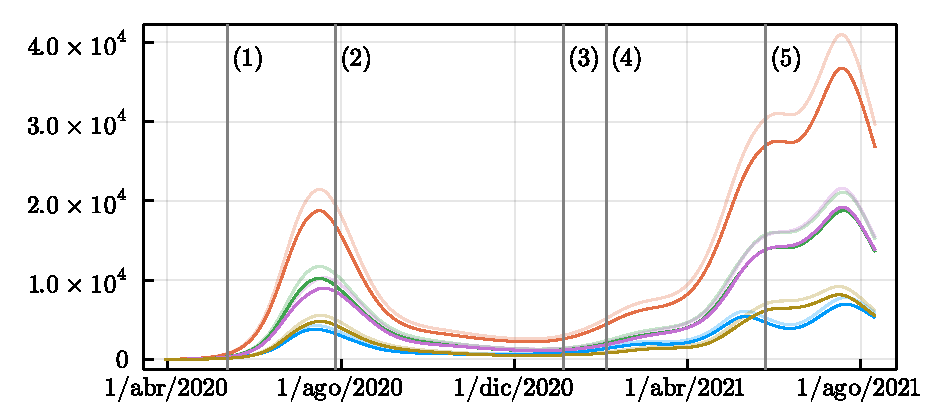
\includegraphics[width=\textwidth]{img/resultados/comparecase_8withnormal_I_gamma_e_0-1724_gamma_i_0-0833_beta_2_2-0000.pdf}
         \caption{Caso \(8\): Cuidado normal y cuarentena fuerte.}
         \label{img:esc-beta-chico-c8}
     \end{subfigure}
     \hfill
    \begin{subfigure}[b]{0.99\textwidth}
    \centering
    \scalebox{0.6}{
    \begin{tikzpicture}
	\begin{pgfonlayer}{nodelayer}
		\node [style=none] (50) at (5, 0) {};
		\node [style=none] (51) at (7, 0) {};
		\node [style=none] (52) at (6, -0.5) {Prioridad Alta};
		\node [style=none] (53) at (2, 0) {};
		\node [style=none] (54) at (4, 0) {};
		\node [style=none] (55) at (3, -0.5) {Prioridad};
		\node [style=none] (56) at (-1, 0) {};
		\node [style=none] (57) at (1, 0) {};
		\node [style=none] (58) at (0, -0.5) {Prioridad};
		\node [style=none] (59) at (-4, 0) {};
		\node [style=none] (60) at (-2, 0) {};
		\node [style=none] (61) at (-3, -0.5) {Prioridad Baja};
		\node [style=none] (62) at (-7, 0) {};
		\node [style=none] (63) at (-5, 0) {};
		\node [style=none] (64) at (-6, -0.5) {Sin Prioridad};
		\node [style=none] (65) at (0, -1) {Media Baja};
		\node [style=none] (66) at (3, -1) {Media Alta};
	\end{pgfonlayer}
	\begin{pgfonlayer}{edgelayer}
		\draw [style=class5] (50.center) to (51.center);
		\draw [style=class1] (62.center) to (63.center);
		\draw [style=class2] (59.center) to (60.center);
		\draw [style=class3] (56.center) to (57.center);
		\draw [style=class4] (53.center) to (54.center);
	\end{pgfonlayer}
\end{tikzpicture}

    }
    \end{subfigure}
        \caption[Personas infectadas para caso hipotéticos seleccionados.]{Personas infectadas para caso hipotéticos seleccionados, con la estimación de los casos reales de fondo. Diferentes límites para el eje \(y\). Las líneas grises corresponden a las fechas relevantes de la tabla \ref{table:fechas-relevantes}.}
        \label{img:hip-3478-I-comp-beta1-2}
\end{figure}
